\documentclass{article}
\usepackage{titling}
\usepackage{lipsum}
\usepackage{amsmath}
\usepackage{listings}
\usepackage{graphicx}
\usepackage{subcaption}
\usepackage{tabularx}



\begin{document}
\noindent
\begin{minipage}[t]{0.6\textwidth}
    \begin{flushleft}
        \LARGE\textbf{CSCI 347 - Project 1} \\
        \vspace{6pt} % add 6pt of vertical space
        \hrule width 10cm
        \vspace{12pt}
        \large\textbf{Preston Duffield} \\
        \large Western Washington University \\
        % \today
        April 12, 2023
        \vspace{24pt}
    \end{flushleft}
\end{minipage}

\section*{Analyzing time with respect to buffer size}

Using filesec to encrypt and decrypt,
we measure the time it takes in seconds for the program to complete with an input text file of 20,227 bytes.
We also record the individual read and write calls the program made during its execution.
A Python program \footnote{See code listing in the Appendix.}
was then written to execute filesec 100 times per buffer size, and the results were exported into a csv file.
That data was then used to create box plots in Minitab to observe trends.



\subsection*{Encrypt}
\begin{figure}[h]
  \centering
  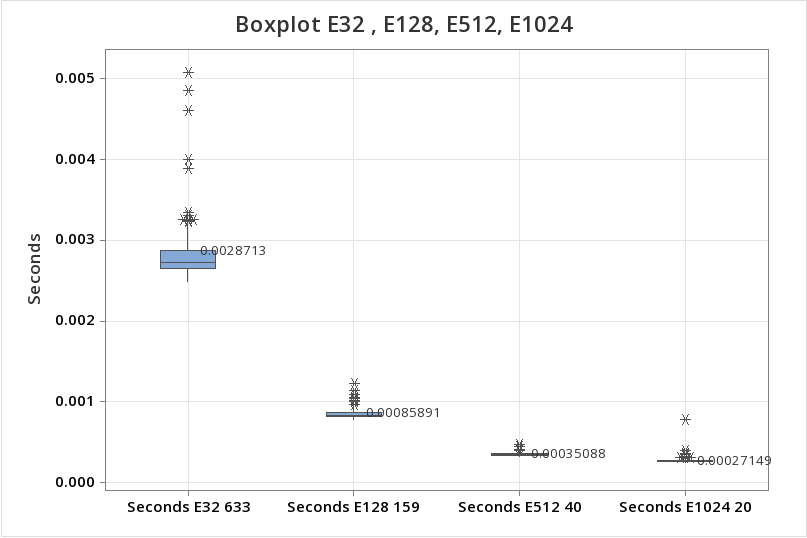
\includegraphics[width=1\textwidth]{./e.png}
  \caption{Minitab output showing the box plot of the time
  in seconds it takes for filesec to encrypt a file.
  Note that the sample mean is shown for each buffer size.}
  \label{fig:equal}
\end{figure}

\clearpage
\subsection*{Decrypt}
\begin{figure}[h]
  \centering
  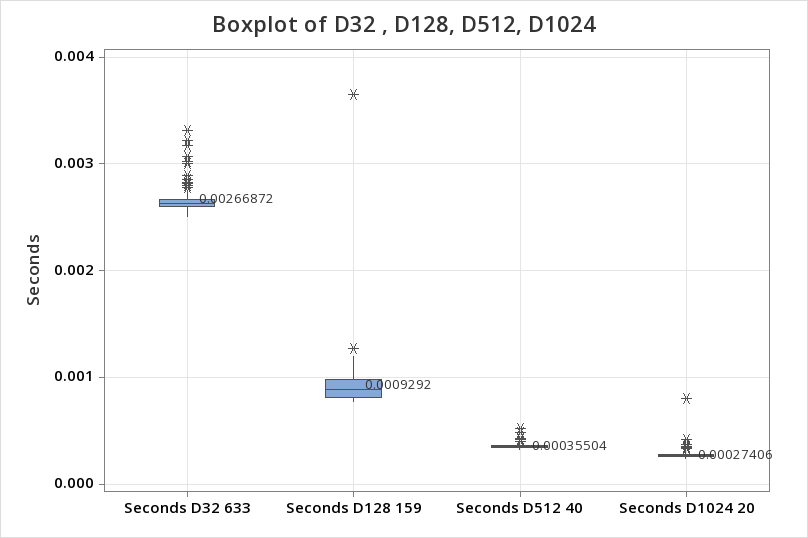
\includegraphics[width=1\textwidth]{./d.png}
  \caption{Minitab output showing the box plot of the time
  in seconds it takes for filesec to Decrypt a file.
  Note that the sample mean is shown for each buffer size.}
  \label{fig:D}
\end{figure}

\subsection*{Table of sample means}
\begin{table}[htbp]
  \begin{tabularx}{\textwidth}{|X|X|X|X|X|}
  \hline
          & 32 & 128 & 512 & 1024 \\
  \hline
  Encrypt & 0.00287 & 0.00085 & 0.00035 & 0.00027 \\
  \hline
  Decrypt & 0.00266 & 0.00092 & 0.00035 & 0.00027 \\
  \hline
  \end{tabularx}
  \caption{The mean runtime of Encrpyt and Decrypt for different buffer sizes, ranging from 32 to 1,024.}
  \end{table}

  We can see that for both Encrpyt and Decrypt, the figures are similar.
  By observing the box plots and the table of mean values, we can conclude that increasing
  the buffer size decreases the runtime of the program.
  However, as the buffer size increases, the rate at which the program speeds up decreases.
  In other words, there is diminishing returns from increasing the buffer size.
  I would hypothesize that at the higher values of the buffer size,
  we are seeing the other apsects of the program in the time it takes to complete.

\clearpage

\section*{Analyzing read and write calls}
\subsection*{Table of read and write calls}
  \begin{table}[htbp]
    \begin{tabularx}{\textwidth}{|X|X|X|X|X|}
    \hline
            & 32 & 128 & 512 & 1024 \\
    \hline
    Encrypt & 633 & 159 & 40 & 20 \\
    \hline
    Decrypt & 633 & 159 & 40 & 20 \\
    \hline
    \end{tabularx}
    \caption{The read/write calls of Encrpyt and Decrypt for different buffer sizes, ranging from 32 to 1,024 on a text file of 20,227 bytes.}
    \end{table}

The program calls to read and write an equal amount of times in all cases, as the calls are subsequent to each other and within the same while loop. 
We can see that the file calls is roughly:
\begin{equation*}
  \text{read/write calls} = \lceil\frac{\text{file size}}{\text{buffer size}} \rceil
  \end{equation*}

  That is, the cieling of the file size divided by the buffer size.
  This is intuitive as the bufffer would be full for all except the last call to read and write.
  This buffer would only be partially filled, but would still incure a call to both read and write.

\clearpage
\appendix
\section*{Appendix}
\begin{lstlisting}[language=Python, 
  basicstyle=\ttfamily\tiny, 
  numbers=left, 
  numberstyle=\tiny, 
  frame=single, 
  caption= {Pyhton code to call filesec an arbitrary amount of times and record the output in a csv file.},
  label=code:my_python_code]
  import subprocess
  import csv
  
  def run_filesec(times, mode, input_file, output_file):
      with open(output_file, 'w', newline='') as csvfile:
          # fieldnames = ['Read calls', 'Write calls', 'Elapsed time']
          fieldnames = ['Elapsed time (Seconds)']
          writer = csv.DictWriter(csvfile, fieldnames=fieldnames)
          writer.writeheader()
  
          for i in range(times):
              result = subprocess.run(['./filesec', mode, input_file], capture_output=True, text=True)
              output = result.stdout.strip().split('\n')
              
              # read_calls = int(output[0].split(': ')[1])
              # write_calls = int(output[1].split(': ')[1])
              elapsed_time = float(output[2].split(': ')[1].split(' ')[0])
  
              writer.writerow({'Elapsed time (Seconds)': elapsed_time})
  
  if __name__ == '__main__':
      # Number of times to run the C program
      times = int(input("Enter the number of times to run the C program: "))
  
      # Mode: "-e" or "-d"
      mode = input("Enter the mode (-e or -d): ")
  
      # Input file
      input_file = input("Enter the input file name: ")
  
      # Output CSV file
      output_file = "output.csv"
  
      run_filesec(times, mode, input_file, output_file)
  
\end{lstlisting}


\end{document}
